% \documentclass[a4paper]{article}
\documentclass[9pt,technote]{IEEEtran}

\usepackage[utf8]{inputenc}
\usepackage[T1]{fontenc}
\usepackage{graphicx}
\usepackage{hyperref}
\usepackage{amsmath}
\usepackage{amssymb}
\usepackage{amsthm}
\usepackage{mathenv}
\usepackage{multirow}
\usepackage{breqn}


\DeclareMathAlphabet{\itbf}{OML}{cmm}{b}{it}

% numérotation au sein de chaque section (du style "2.1")
\numberwithin{equation}{section}

% commandes perso
\newcommand{\R}{\mathbb{R}}
\newcommand{\ie}{\emph{i.e.} }
\newcommand{\RnX}{\mathbb{R}_n[X]}
\newcommand{\N}{\mathbb{N}}
\newcommand{\C}{\mathcal{C}}
\newcommand{\Ccinf}{\mathcal{C}_c^{\infty}}
\newcommand{\Cinf}{\mathcal{C}^{\infty}}
\newcommand{\supp}{\textrm{supp}}
\newcommand{\bx}{\mathbf{x}}
\newcommand{\bv}{\mathbf{v}}
\newcommand{\Mbv}{M_{\mathbf{v}}}
\newcommand{\Tbv}{T_{\mathbf{v}}}
\newcommand{\mubv}{\mu_{\mathbf{v}}}
\newcommand{\sbv}{s_{\mathbf{v}}}
\newtheorem{definition}{Definition}
\newtheorem{lemma}{Lemma}
\newtheorem{theorem}{Theorem}

\title{Consistency of Fanbeam Projections of a Translating Object Along an Arc of a Circle}
\author{Thomas Boulier, Rolf Clackdoyle, Jérôme Lesaint, Laurent Desbat}
\date{}

\begin{document}

\maketitle

\begin{abstract}
In this article, we compute data consistency conditions (DCCs) in the case of a translating object illuminated by a fan-beam source which is moving along an arc of a circle. The DCCs are thus a variation of thoses computed in~\cite{clackdoyle2015consistency}, where the object remained still. In a second part, we use the DCCs in order to retrieve the velocity of the object. These results are illustrated by numerical examples.
\end{abstract}

\section{Introduction}

In the field of CT-imaging, data consistency conditions (DCCs) use the redundancy of the data in order to establish relations that must be fulfilled. These conditions are called \emph{full} when they are necessary and sufficient. One of the best known DCCs are the Helgason-Ludwig (H-L) conditions~\cite{helgason1980radon,ludwig1966radon}, which are full and are applied in the case of parallel projections along a line.

In~\cite{clackdoyle2015consistency}, the H-L conditions are modified to the case of a source moving along an arc of a circle. In brief, they integrated all rays passing through the same point along a "virtual" line between the two extreme positions of the source. The H-L conditions could then be applied; numerical examples showed a situation where attenuation was added, and the DCCs permitted to recover this attenuation coefficient. The case of a moving object has been tackled in~\cite{yu2006data,yu2007data}, where the authors use the H-L conditions in the case of an object undergoing rigid body motion while illuminated by a fan-beam source along a line. Those conditions allow the authors to recover the parameters of the movement, in order to suppress the artifacts caused by such movement.

In this article, we will be interested by those two situations. We will suppose that an object is translating while illuminated by a fan-beam source which is moving along an arc of a circle. Using a change of frame, we will use the same idea as in~\cite{clackdoyle2015consistency} for the derivation of DCCs. Then, in a second part, we will use the DCCs for the recovery of the velocity of translation, in order to correct motion artifacts.

\section{Theory} 
\label{sec:theory}

\subsection{Problem under consideration}
\label{sub:problem_under_consideration}

Let us begin with some notations and definitions. We will consider an object in $\R^2$ to be imaged by a fanbeam source that follows an arc of circle with center $O$ and radius $R_0$ (see Figure~\ref{fig:notations}, left). The object will be identified with its density function $\mathbf{x} \mapsto \mu(\mathbf{x}) \in \Ccinf(\R^2)$.
\begin{figure}[!ht]
	\centering
	\begin{tabular}{c}
	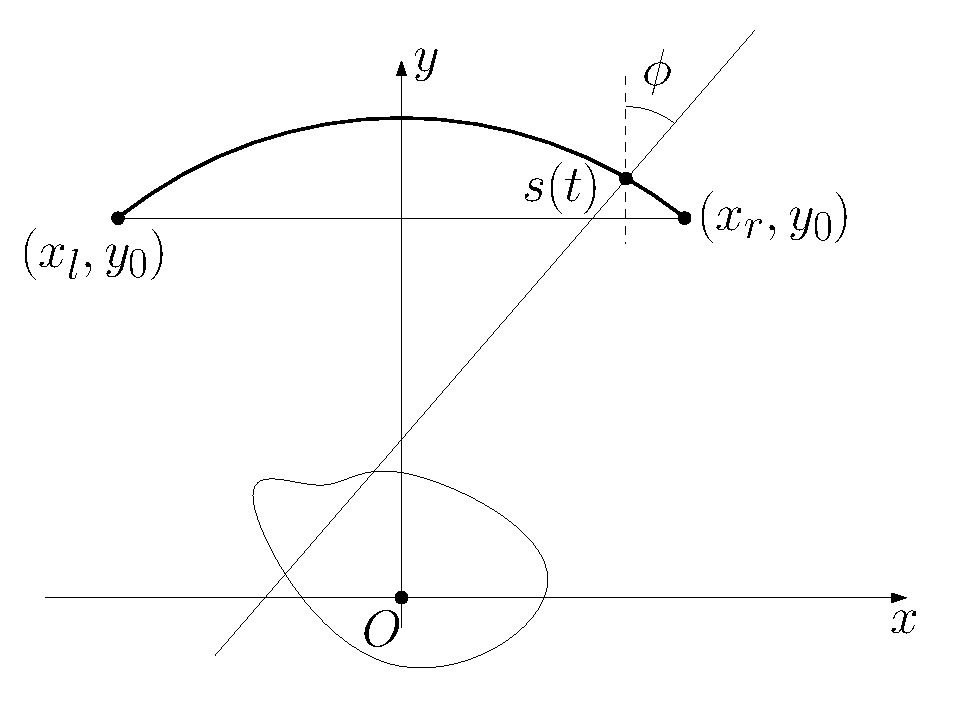
\includegraphics[width=7cm]{figs/frame_scanner_still.eps} \\
	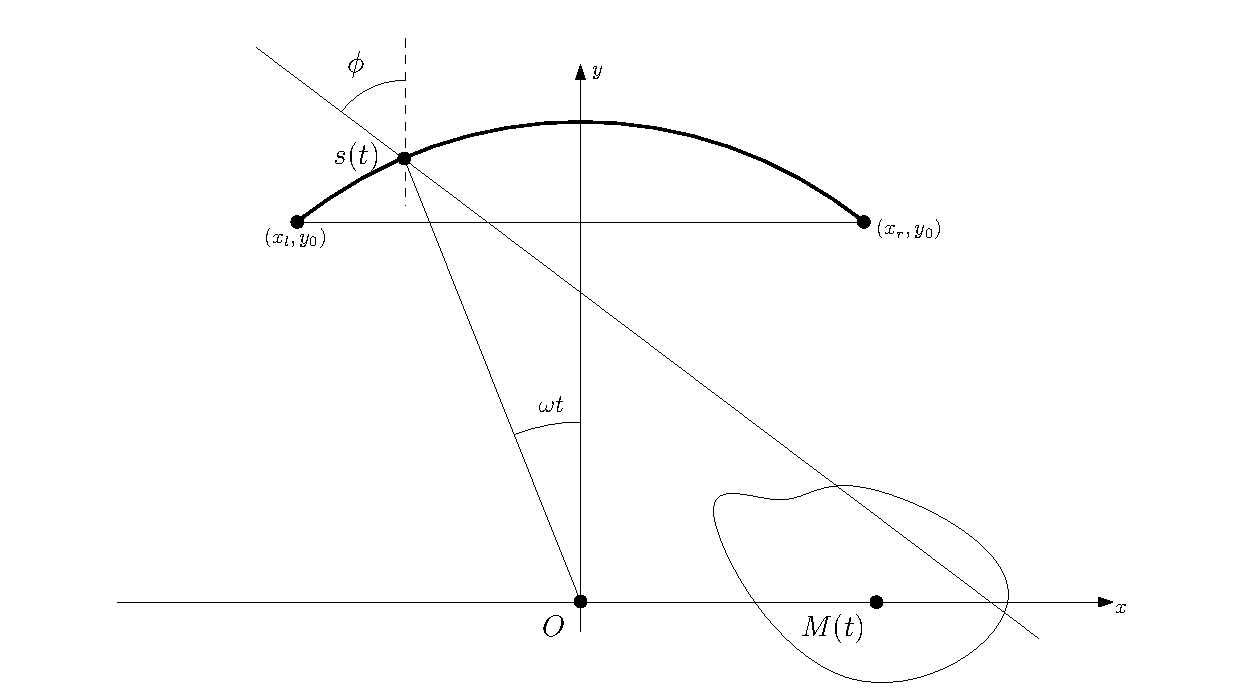
\includegraphics[width=7cm]{figs/frame_scanner.eps}
	\end{tabular}
	\caption{Problem under consideration. The source point $s(t)$ follows the arc of circle depicted in bold. This latter has center $O$ and radius $R_0$.\label{fig:notations}}
\end{figure}
The angular velocity of the source will be denoted $\omega$, and the time $t$ will range from $-T/2$ to $T/2$, where $T>0$. Hence, if we denote $s(t)$ the position of the source at time $t$, one has
\begin{equation}
	s(t) = \left( -R_0 \sin(\omega t), R_0 \cos(\omega t) \right).
\label{eq:source_position}
\end{equation}
Furthermore, we will denote $s(T/2)=(x_l,y_l)$ (resp. $s(-T/2)=(x_r,y_r)$) the extreme left (resp. right) position of the source. Since $y_l = y_r = R_0 \cos(\omega T/2)$, we will call $y_0$ this common value. In the following, we will suppose that $\supp(\mu)$ lies in the half-space $\{ y < y_0 \}$, and that $y_0 > 0$ (\ie $0 < \omega T < \pi$).

We will suppose that at any time $t$ rays are simultaneously emitted from the source $s(t)$ with angle $\phi$ ranging from $-\pi/2$ to $\pi/2$. With this setup in mind, we can define the operator giving the acquired data from the object.
\begin{definition}
The \emph{fanbeam projection data} of an object with density function $\mu$ is a function $(t,\phi) \mapsto T\mu(t,\phi)$ defined by
\begin{equation}
	(T\mu)(t,\phi) = \int_0^{+\infty} \mu \left( s(t) + l \left[ \sin \phi, -\cos \phi \right] \right) dl,
\end{equation}
where $t \in \left[ -T/2, T/2\right]$, $\phi \in \left[ -\pi/2, \pi/2\right]$ and $s(t)$ is given by~(\ref{eq:source_position}). The operator $\mu \mapsto T\mu$ is called the \emph{fanbeam projection operator}.
\end{definition}


Now let us suppose that the object is translating along a line with a constant velocity vector $\bv = (v_1, v_2)\in \R^2$ (see Figure~\ref{fig:notations}, right). In other words, if we denote $\Mbv(t)$ its center of mass at any time $t$, we have
\begin{equation}
	\Mbv(t) =  \left( \left( t + \frac{T}{2} \right)v_1, \left( t + \frac{T}{2} \right)v_2 \right)
\label{eq:center_of_mass}
\end{equation}
The density function of the object now depends on both the space variable $\bx \in \R^2$ and the time $t$. If we denote it $\mubv$, we have
\begin{equation}
	\mubv(t,\bx) = \mu\left( \bx - \Mbv(t)\right).
\end{equation}
In this regard, the fanbeam projection data will be modified in the following way.
\begin{definition}
The \emph{fanbeam projection data of a translating object} with density function $\mu$ and translating velocity vector $\bv$ is given by
\begin{equation}
	(\Tbv\mu)(t,\phi) = \left( T \mubv(t,\cdot) \right)(t,\phi).
\label{eq:def_Tv}
\end{equation}
\end{definition}

The aim of this note is to derive data consistency conditions (DCCs) from~(\ref{eq:def_Tv}), in order to retrieve the velocity vector $\bv$ from the knowledge of $\Tbv$.

\subsection{Derivation of DCCs}

In order to derive DCCs, we will first change our frame of reference, from $\left(O, x, y\right)$ to $\left(M(t), x', y'\right)$, so that the object is at the center and the line between the start point and the end point of the source is still parallel to the $x'$-axis (see Figure~\ref{fig:change_frame}, right). In other words, we are performing the following change of variables
\begin{equation}
	(x,y) \leftrightarrow (x',y') = \mathcal{R}_{\beta} \left( (x,y)-\Mbv(t) \right),
\end{equation}
where $\mathcal{R}_{\beta}$ is the rotation of angle $\beta$. This latter is the angle depicted in Figure~\ref{fig:change_frame} (left) and is given by
\begin{equation}
	\beta = \arctan \left( \frac{T v_2}{2R_0 \sin(\omega T/2) + T v_1} \right).
\end{equation}

\begin{figure}[!ht]
	\centering
	%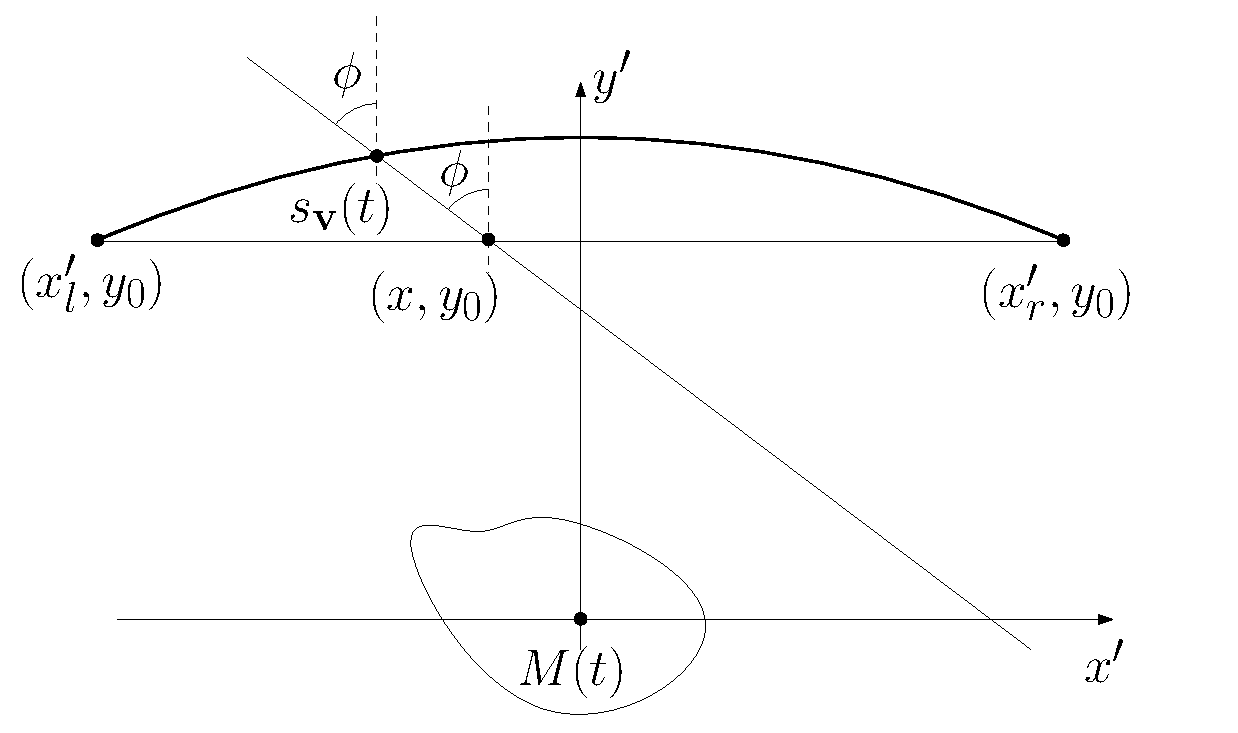
\includegraphics[width=12cm]{figs/frame_object.eps}
	\begin{tabular}{c}
	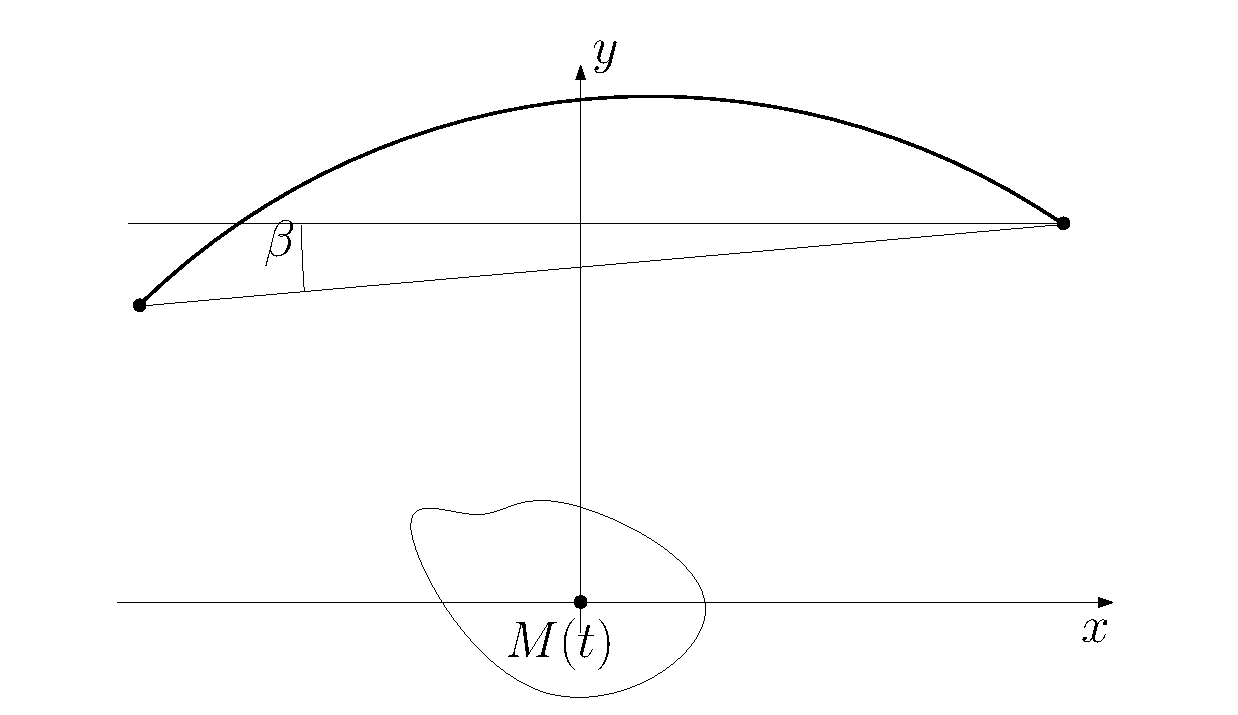
\includegraphics[width=7cm]{figs/frame_object_before_rotation.eps} \\
	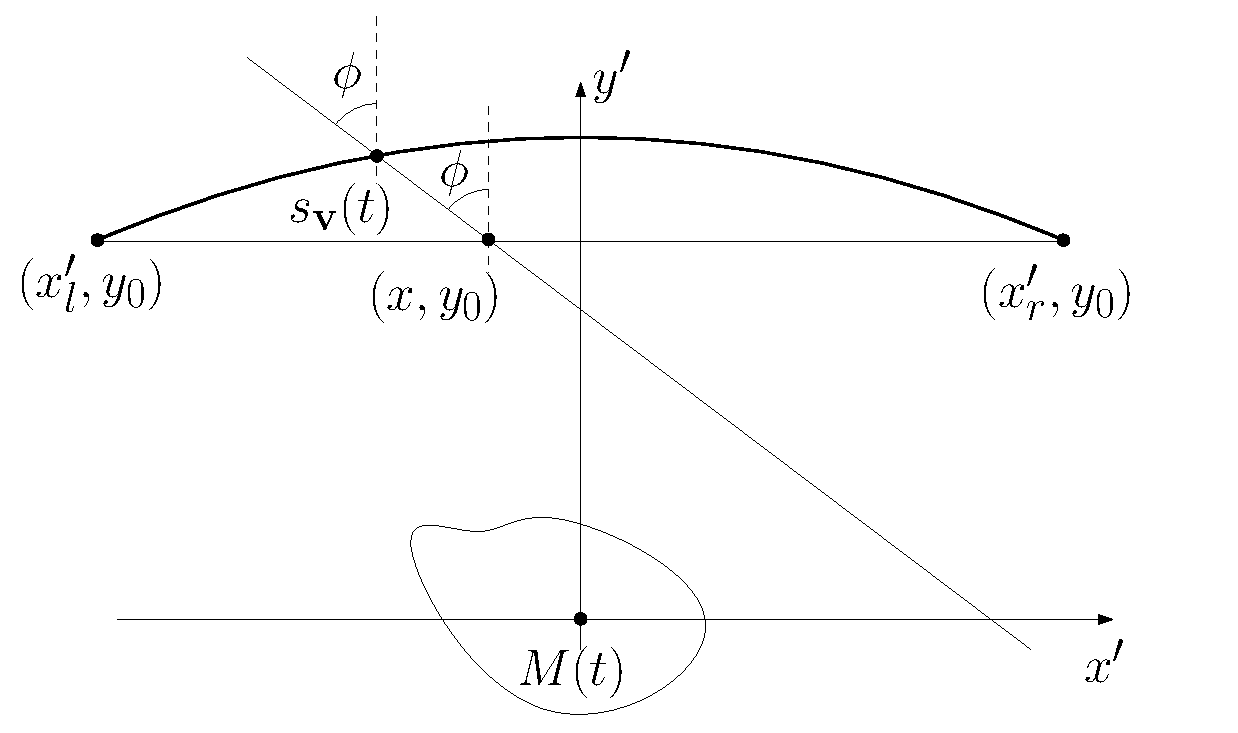
\includegraphics[width=7cm]{figs/frame_object.eps}
	\end{tabular}
	\caption{Change of frame: the object is now at center of the coordinates system. Left, only translation of the center of frame; right, after rotation of angle $\beta$. Note that the angle $\phi$ is the same as in Figure~\ref{fig:notations}, right.\label{fig:change_frame}}
\end{figure}

In this frame, the coordinates of the source are given by $\sbv(t)=\mathcal{R}_{\beta} \left( s(t)-\Mbv(t) \right)$. With this in mind, the data is given by the following formula
\begin{equation}
	(\Tbv\mu)(t,\phi) = \int_0^{+\infty} \mu' \left( s_{\bv}(t) + l \left[ \sin \phi, -\cos \phi \right] \right) dl,
\end{equation}
where $\mu'(\bx')=\mu(\bx)$, \ie the function $\mu'$ takes its arguments from the space $\left(M(t), x', y'\right)$.

In other words, we are now dealing with a fixed object whose density function is given by $\mu'$ illuminated by a source following an arc of a cycloid in the frame $\left(M(t), x', y'\right)$ (see Figure~\ref{fig:change_frame}, right).

Here, the extreme points $\sbv(-T/2)$ and $\sbv(T/2)$ have the same $y'$-coordinate $y'_0$. We will call $x'_l$ (resp. $x'_r$) the $x'$-coordinates of $\sbv(T/2)$ (resp. $\sbv(-T/2)$). This allows us to define what we call the \emph{virtual fanbeam projection} from a point $(x',y'_0)$.
\begin{definition}
	For any point $x'$ between $x'_l$ and $x'_r$, for any angle $\phi \in \left[ -\pi/2, \pi/2\right]$, the \emph{virtual fanbeam projection} of the object $\mu$ is defined by
\begin{equation}
	\left( \tilde{T}\mu	\right)(x',\phi) = \int_0^{+\infty} \mu \left( (x',y'_0) + l \left[ \sin \phi, -\cos \phi \right] \right) dl.
\end{equation}
This is called \emph{virtual} since it does not correspond to an actual position of the source.
\end{definition}

In the following lemma, we will make a connection between the virtual fanbeam projection and the fanbeam projection of the translating object.
\begin{lemma}
	Let us fix a time $t \in \left[ -T/2, T/2\right]$ and an angle $\phi \in \left[ -\pi/2, \pi/2\right]$. Let us define
	\begin{equation}
		x' = s_{1,\bv}(t) + \tan \phi \left( s_{2,\bv}(t) - y'_0 \right),
	\end{equation}
	where, for any time $t$, $\left( s_{1,\bv}(t), s_{2,\bv}(t) \right)$ are the coordinates of $\sbv(t)$.
	Then, one has
	\begin{equation}
		\left( \tilde{T}\mu	\right)(x',\phi) = \left( \Tbv \mu \right)(t,\phi).
	\end{equation}
\label{lem:T_x_t}
\end{lemma}

We can now define what are the DCCs of our problem.
\begin{theorem}
Let us fix a density function $\mu$. For any integer $n$, there exist a function $(x',t)\mapsto W_{n,v}(t,x') \in \Cinf \left( [-T/2,T/2] \times [x'_l,x'_r] \right)$ such that the function $B_n$ defined by
\begin{equation}
	B_n := x' \mapsto \int_{-T/2}^{T/2} \left( \Tbv \mu \right)\left( t,\lambda(t) \right) W_n(x',t,v) dt,
\label{eq:DCC}
\end{equation}
is a polynom of order $n$. In the formula above, the angle $\lambda(t)$ is defined by
\begin{equation}
	\lambda(t) = \arctan \left( F(x',t,\bv) \right),
\end{equation}
where $F(x',t,\bv)$ is defined as a fraction $A/B$ with
\begin{dmath}
	A = x' + \cos \beta \left( R_0 \sin(\omega t) + \left( t + \frac{T}{2} \right)v_1 \right) + \\
	\sin \beta \left( R_0 \cos(\omega t) - \left( t + \frac{T}{2} \right)v_2 \right)
\end{dmath}
and
\begin{dmath}
	B = \cos \beta \left( R_0 \cos(\omega t) - \left( t + \frac{T}{2} \right)v_2 \right) - \sin \beta \left( R_0 \sin(\omega t) + \left( t + \frac{T}{2} \right)v_1 \right) - y'_0 
\end{dmath}
Moreover, it is possible to derive $W_{n,v}(t,x')$ analytically using the following formula
\begin{equation}
	W_{n,v}(t,x') = \tan^n F(x',t,\bv) \cos F(x',t,\bv) \frac{\partial F}{\partial t} (x',t,\bv)
\end{equation}
\end{theorem}

Although the formula giving $W_{n,v}(t,x')$ is quite heavy, we can observe that in the case $v_1=v_2=0$, we obtain the formula (7) in~\cite{clackdoyle2015consistency} since
\begin{equation}
	F \left( x',t,\bv = (0,0) \right) = \frac{x' + R_0 \sin(\omega t)}{R_0 \cos(\omega t)}
\end{equation}

\section{Numerical simulations}

\subsection{Principles}
\label{sub:principles}
Let us suppose that we have the projections $\left( \Tbv \mu \right)(t,\phi)$. In order to recover $v$, we can perform the following optimization procedure. Since $B_n(x')$ in equation~(\ref{eq:DCC}) is supposed to be a polynom of order $\leq n$, one can minimize
\begin{equation}
	\mathcal{J}(v) = \sum_n \Vert \textrm{res} \left( B_n(\cdot,v) \right) \Vert^2
\end{equation}
with respect to $v$, where $\textrm{res}$ is the residual of the projection onto $\R_n[X]$. This will give us the velocity $v$ using only the knowledge of the data $\left( \Tbv \mu \right)(t,\phi)$.

\subsection{Application}
\label{sub:application}
Here, we will consider an object translating along the $x$-axis, \ie $v_2=0$. The object under consideration is an ellipse of uniform density, whose axis are $30$ and $15$ millimeters respectively. The source is rotating around the object with radius $R_0 = 600 \, \textrm{mm}$, with angle velocity $\omega = 1 \, \textrm{rad} \cdot \textrm{s}^{-1}$. With a velocity of the ellipse given by $v_1 = 0.3 \textrm{mm} \cdot \textrm{s}^{-1}$, we obtain the sinogram depicted in Figure~\ref{fig:sinogram}.
\begin{figure}[!ht]
	\centering
	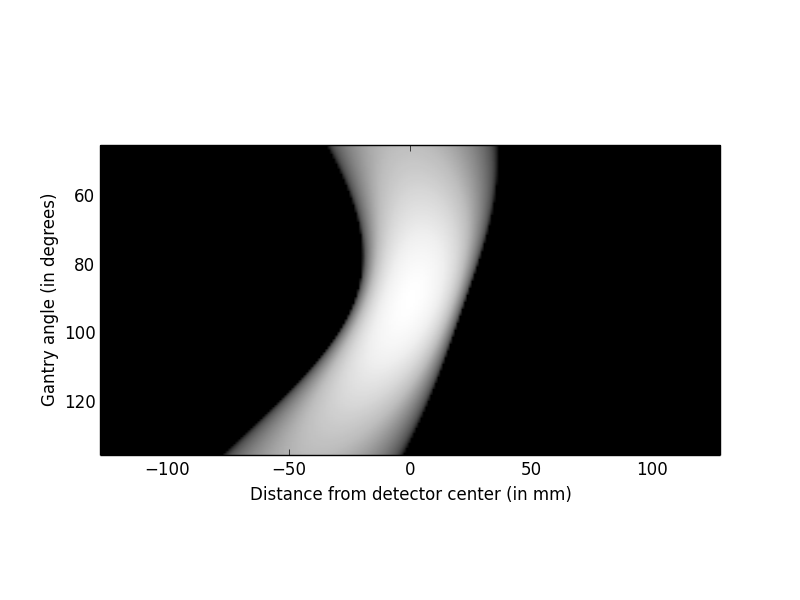
\includegraphics[width=7cm]{figs/sinogram.png}
	\caption{Sinogram of a moving ellipse, with semi-axis $a = 30$ and $b = 15$, translating along the $x$-axis with velocity $v_1 = 0.3$. It is illuminated by a source at distance $R_0 = 600$, rotating with angle velocity $\omega = 1$.\label{fig:sinogram}}
\end{figure}

With this configuration in mind, the functions $x' \mapsto B_n(x')$ for $n = 0,1,2,3$ can be visualized in Figure~\ref{fig:Bnx}.
\begin{figure}[!ht]
	\centering
	\begin{tabular}{c}
	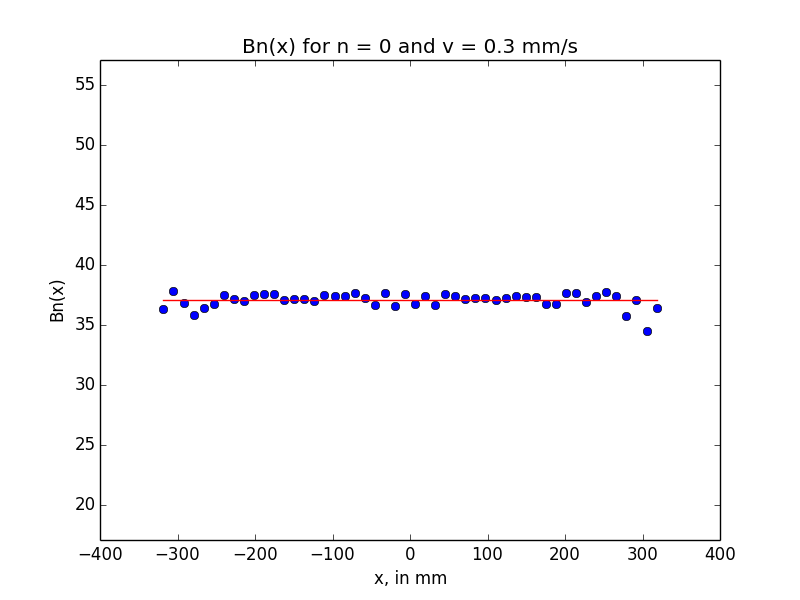
\includegraphics[width=7cm]{figs/B0.png} \\
	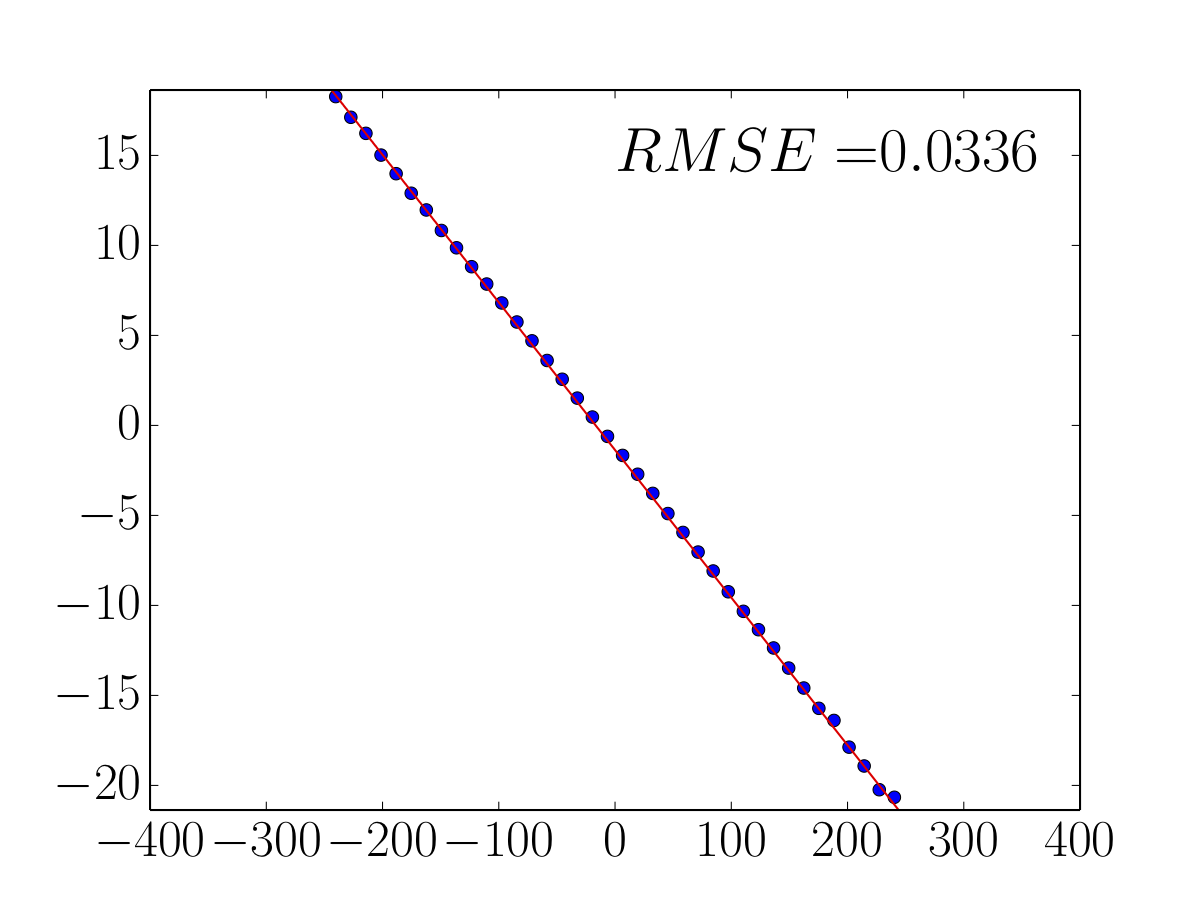
\includegraphics[width=7cm]{figs/B1.png} \\
	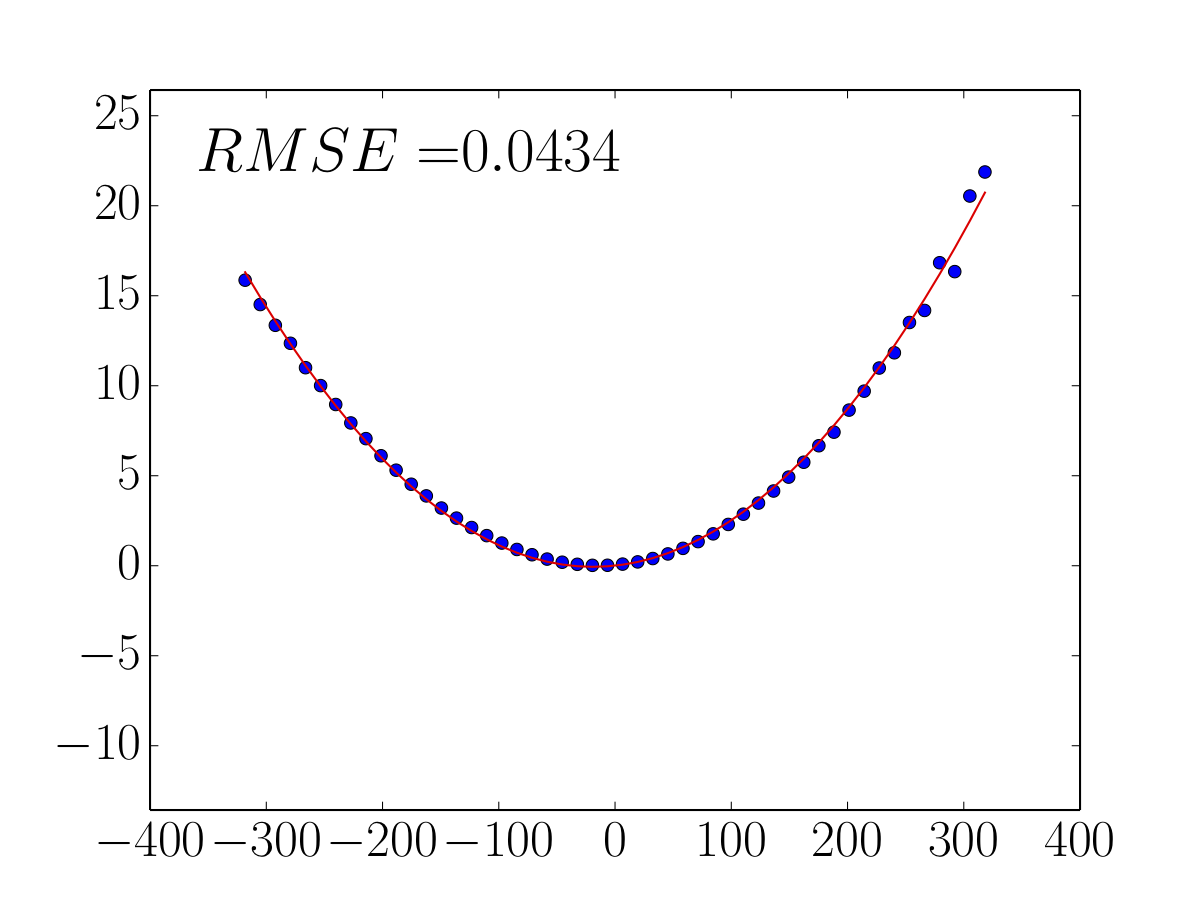
\includegraphics[width=7cm]{figs/B2.png} \\
	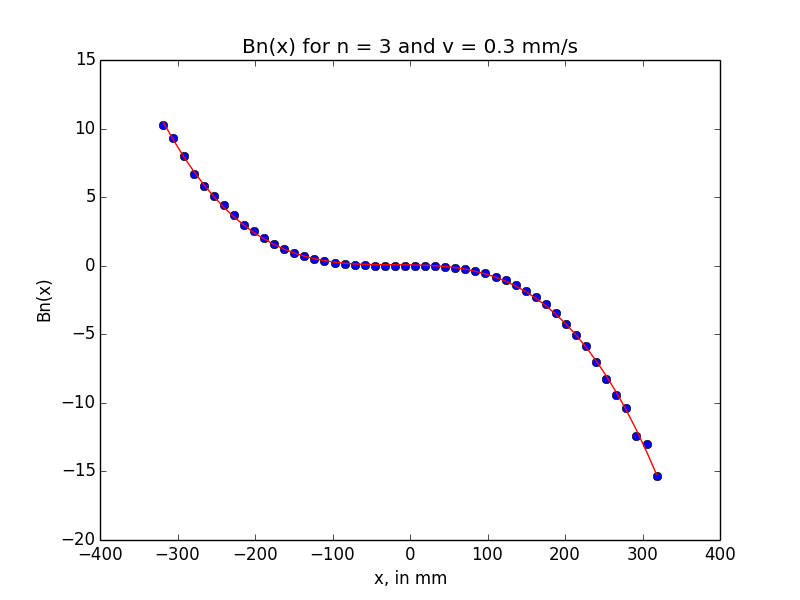
\includegraphics[width=7cm]{figs/B3.png} 
	\end{tabular}
	\caption{From top to bottom, functions $x' \mapsto B_n(x')$ for $n = 0,1,2,3$ respectively.\label{fig:Bnx}}
\end{figure}



\bibliographystyle{plain}
\bibliography{DCC_translation}


\end{document}

